\subsection{Small-scale evaluations}
\label{sec:small-scale}

To assess baseline performance metrics of the designed Interest flooding attack mitigation methods, we evaluated them first using a simplistic small-scale binary tree topology (Fig.~\ref{fig:small-scale}).
All links in this topology were assigned 10~Mbps bandwidths with randomized propagation delays from the range from one to ten milliseconds.
Both legitimate users and attackers were placed only on leaf nodes (red), each expressing Interests towards a single producer placed at the root of the tree. 
% Alex: should we mention that?
The main reason to chose a binary tree topology was that it represents one of the worst cases to defend against flooding DDoS attacks.
That is, sharing of the network links exponentially increases as decreasing level of the binary tree.

\begin{figure}[htbp]
  \centering
  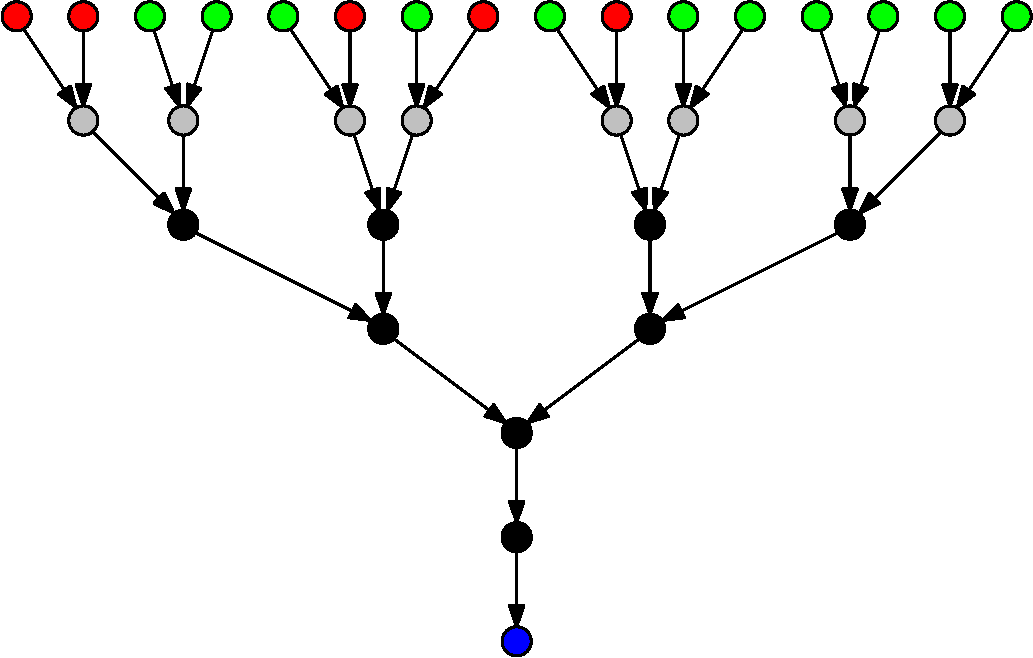
\includegraphics[scale=0.2]{topo-tree-evil-5-good-0-producer-gw}
  \caption{Small-scale binary tree topology}
  \label{fig:small-scale}
\end{figure}


\begin{figure}[htbp]
  \centering
  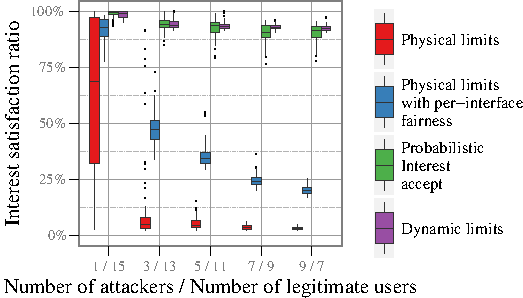
\includegraphics[scale=1]{tree-topo-var-evils-max-consumers-30mins/tree-good-0-producer-gw-avg-1-min}
  \caption{Average consumer Interest satisfaction ratios (first minute)}
  \label{fig:small-scale-topo 1}
\end{figure}


\begin{figure}[htbp]
  \centering
  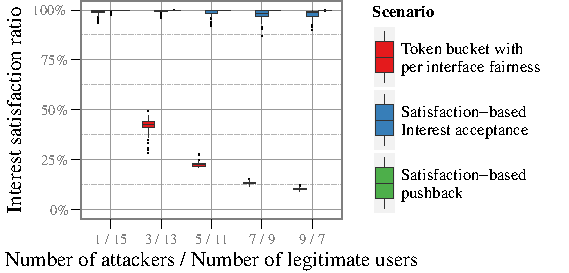
\includegraphics[scale=1]{tree-topo-var-evils-max-consumers-30mins/tree-good-0-producer-gw-avg-1-min-after-1-min}
  \caption{Average consumer Interest satisfaction ratios (second minute)}
  \label{fig:small-scale-topo 2}
\end{figure}

\begin{figure*}[t]
  \centering
  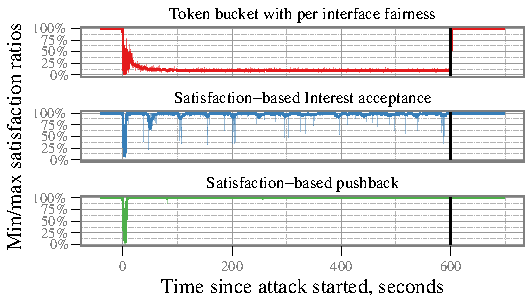
\includegraphics[scale=1]{tree-topo-var-evils-max-consumers-30mins/tree-good-0-producer-gw}
  \caption{Satisfaction ratio dynamics during the attack (7 attackers / 9 legitimate)}
  \label{fig:small-scale-topo 3}
\end{figure*}



%%% Local Variables: 
%%% mode: latex
%%% TeX-master: "paper"
%%% End: 
